% Requires graphicx. Compile from Theory_Comparison or set graphicspath accordingly.
\begin{figure}[htbp]\centering
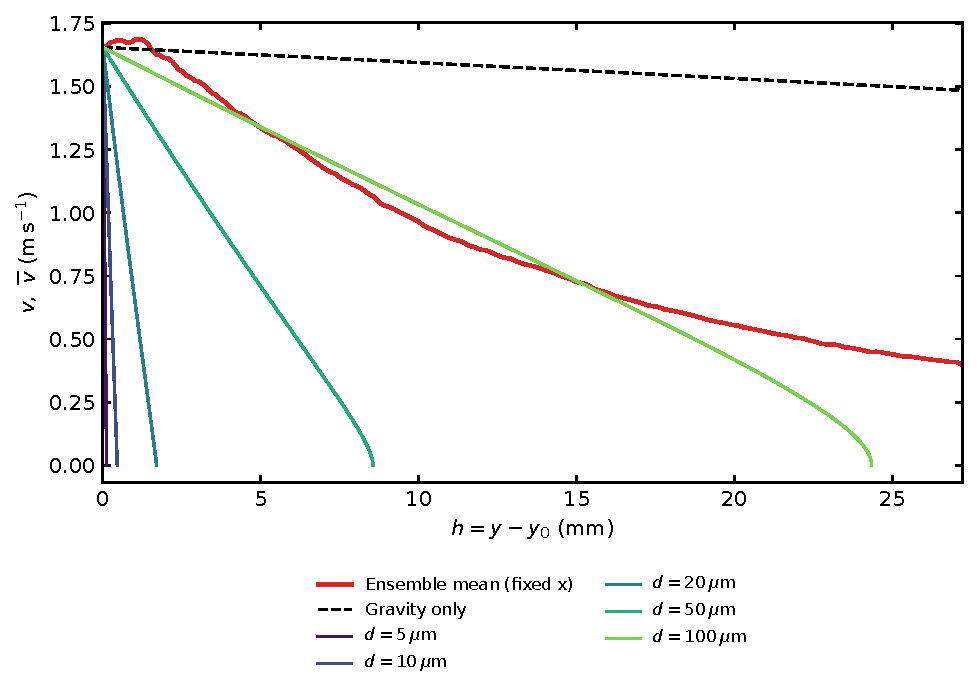
\includegraphics[width=0.92\linewidth]{velocity_reference_full.pdf}
\caption{Fixed-line ensemble-mean axial droplet velocity (red) and individual spherical-droplet reference trajectories in assumed stationary air, with assumed diameters $d=5$, 10, 20, 50 and $100\,\mu\mathrm{m}$. The dashed curve is the gravity-only reference. Height $h=y-y_0$ starts at the first measurement used for initialisation, not the atomiser surface. The ensemble mean is neither a particle trajectory nor a tracked plume centreline. Reference curves stop at their upward turning point or the measurement boundary; no diameter is inferred from agreement.}
\label{fig:velocity-reference-full}
\end{figure}

\begin{figure}[htbp]\centering
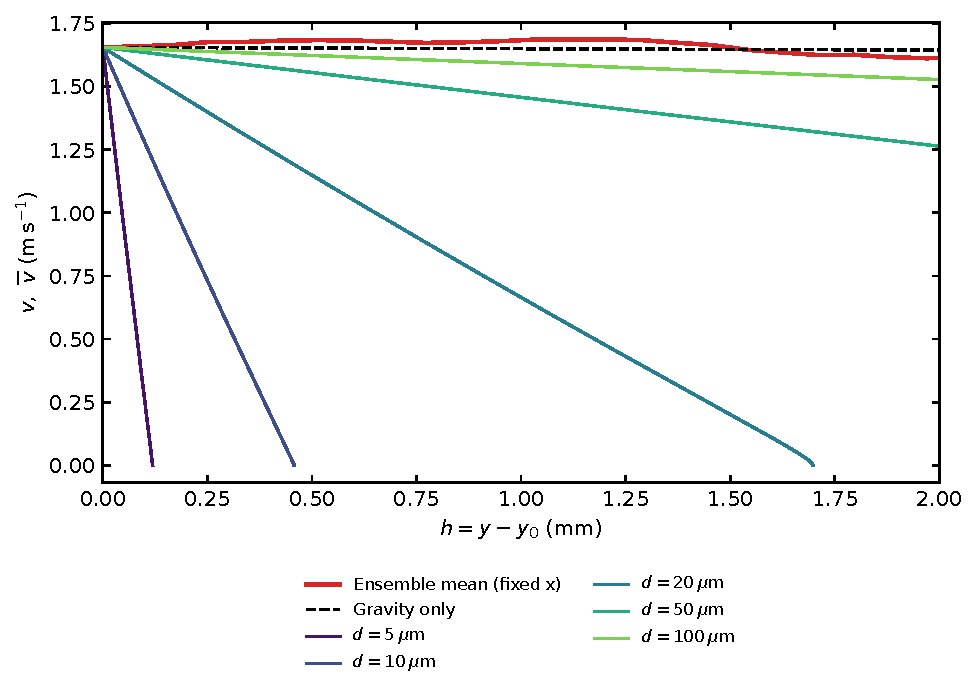
\includegraphics[width=0.92\linewidth]{velocity_reference_near_origin.pdf}
\caption{Near-origin view, $0\leq h\leq2\,\mathrm{mm}$, of exactly the same data and reference curves, colours and line styles as the full-range velocity figure. The small-droplet stationary-air branches are resolved without altering their measured initial velocity, extending stopped droplets, or adding descending branches. Assumed diameters are sensitivity cases.}
\label{fig:velocity-reference-near-origin}
\end{figure}

\begin{figure}[htbp]\centering
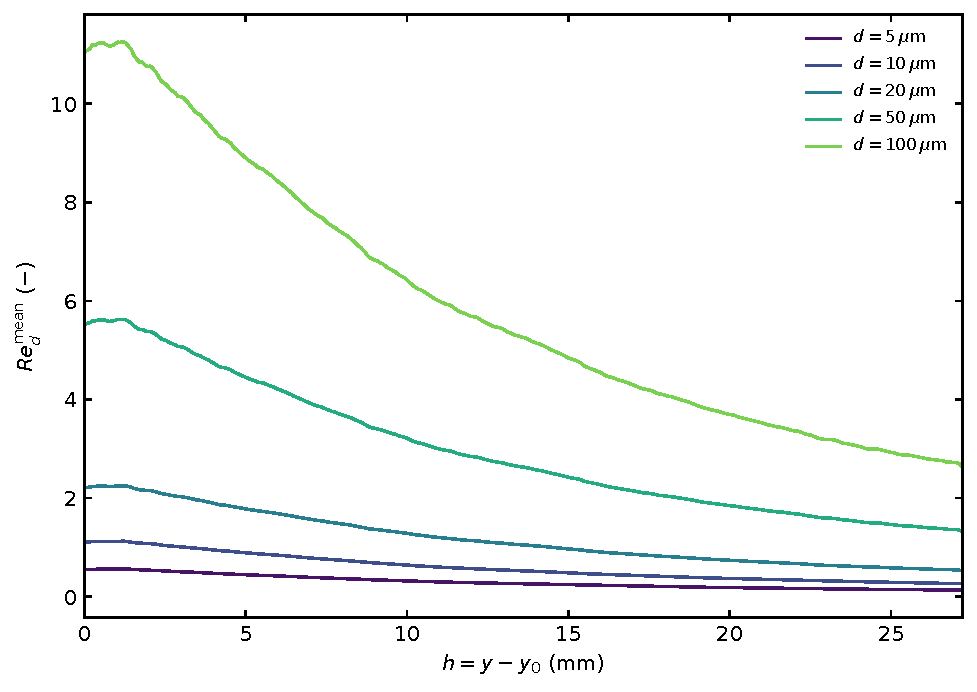
\includegraphics[width=0.92\linewidth]{reynolds_measured_velocity_assumed_air.pdf}
\caption{Conditional in-plane Reynolds estimates $Re_d^{\mathrm{mean}}=\rho_a d\sqrt{\overline{u}^{\,2}+\overline{v}^{\,2}}/\mu_a$ using the measured ensemble-mean droplet vector, assumed stationary air and assumed diameters. This is Reynolds number based on the magnitude of the mean velocity vector, not an ensemble average of instantaneous Reynolds numbers. Curves span the measured domain because their velocities come from the spatial measurements, independently of the trajectory reference endpoints.}
\label{fig:reynolds-measured-velocity-assumed-air}
\end{figure}

\begin{figure}[htbp]\centering
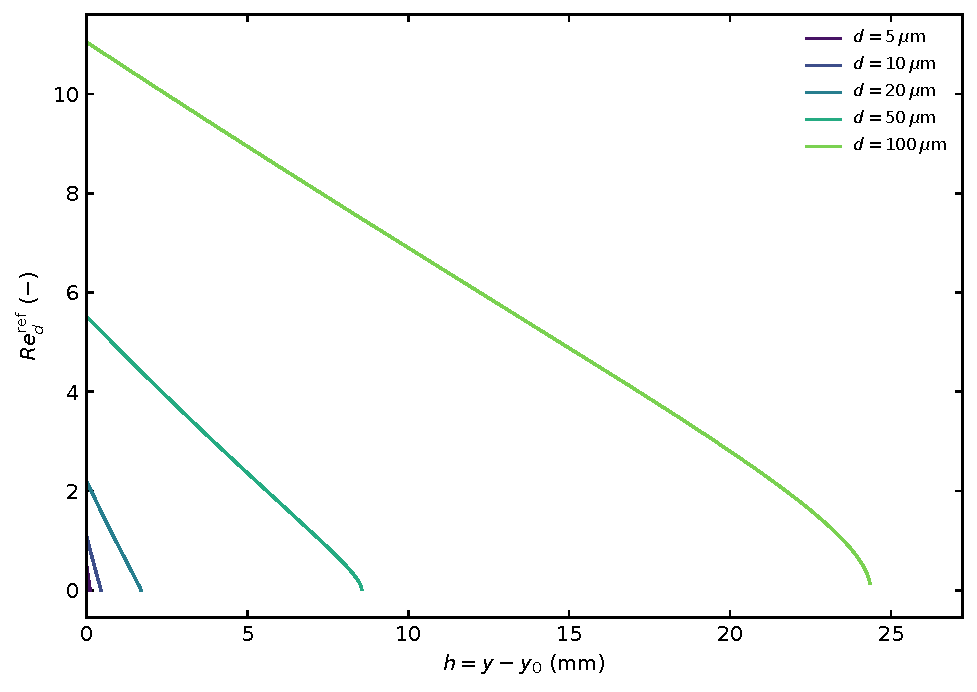
\includegraphics[width=0.92\linewidth]{reynolds_reference_trajectories.pdf}
\caption{Reynolds number $Re_d^{\mathrm{ref}}=\rho_a d\lVert\boldsymbol{w}_a-\boldsymbol{w}_d\rVert/\mu_a$ along each individual reference trajectory in assumed stationary air. Each assumed-diameter curve ends at its own upward turning point or the measurement boundary. These trajectory values are distinct from the conditional estimates based on measured ensemble means; the curves are not extended across the remaining measurement domain.}
\label{fig:reynolds-reference-trajectories}
\end{figure}

\begin{figure}[htbp]\centering
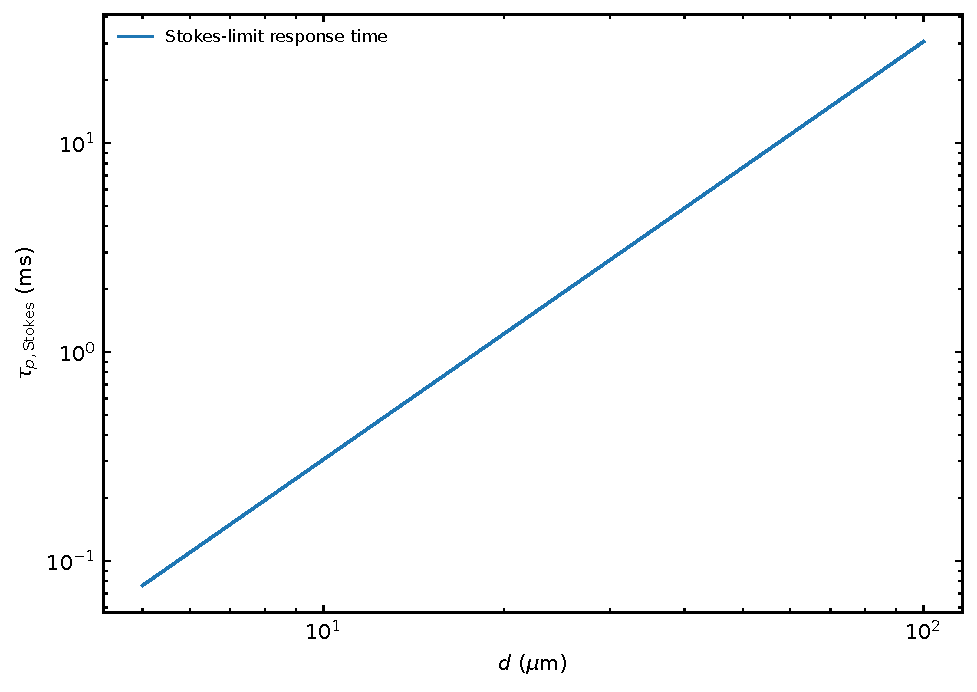
\includegraphics[width=0.92\linewidth]{particle_relaxation_time.pdf}
\caption{Stokes-limit response time $\tau_{p,\mathrm{Stokes}}=\rho_w d^2/(18\mu_a)$ versus assumed droplet diameter, using water and air properties at $20\,^{\circ}\mathrm{C}$. This is a low-Reynolds-number baseline, not an exact finite-Reynolds-number relaxation time. The separately exported $\tau_{\mathrm{drag,sec}}=\tau_{p,\mathrm{Stokes}}/f(Re_d)$ is a drag/slip coefficient timescale.}
\label{fig:particle-relaxation-time}
\end{figure}

\begin{figure}[htbp]\centering
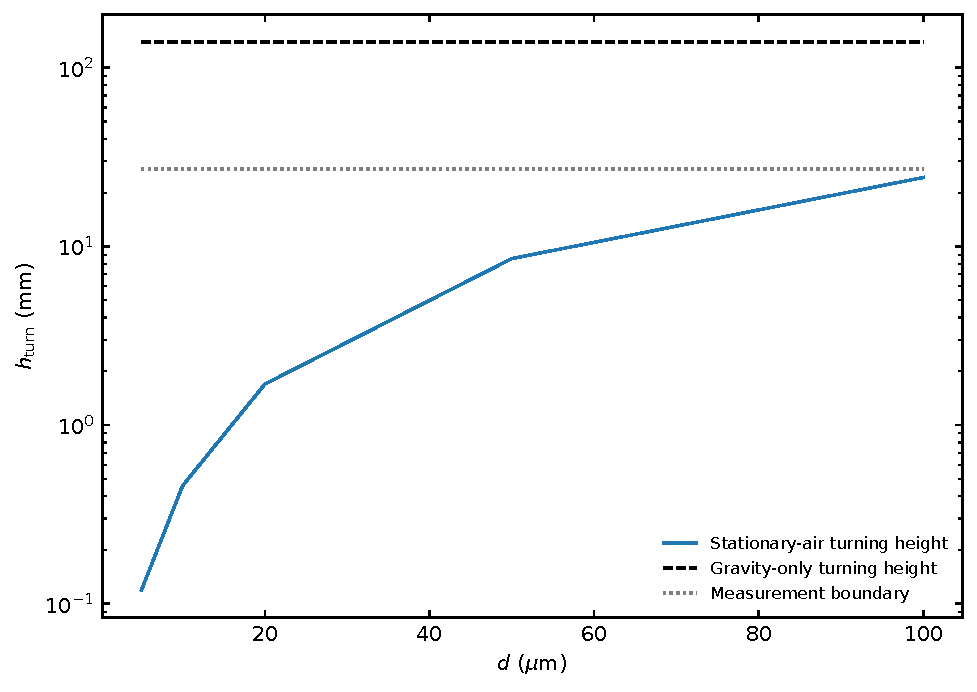
\includegraphics[width=0.92\linewidth]{diameter_sensitivity.pdf}
\caption{Actual upward turning heights of the stationary-air droplet references and the gravity-only reference, measured from the initialisation sample. The dotted line marks the upper measurement boundary, which is a plotting limit rather than a stopping height. The logarithmic ordinate distinguishes the assumed-diameter cases. Actual turning heights and domain-truncated plot endpoints are exported separately.}
\label{fig:diameter-sensitivity}
\end{figure}

\begin{figure}[htbp]\centering
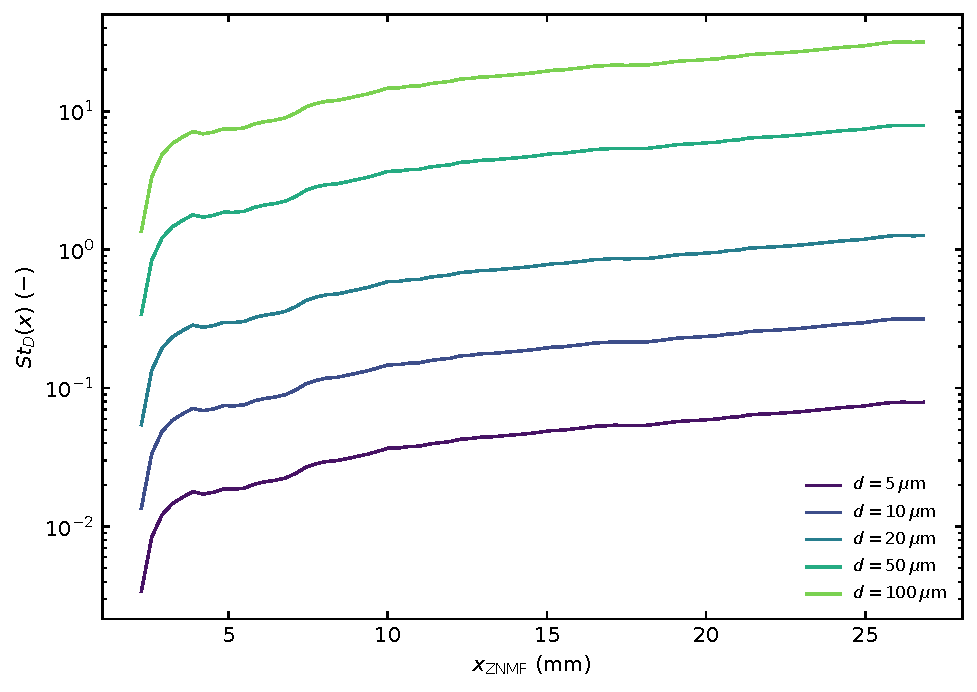
\includegraphics[width=0.92\linewidth]{Jet_Interaction_Sensitivity/znmf_local_nozzle_stokes.pdf}
\caption{Hypothetical jet-interaction sensitivity $St_D(x)=\tau_{p,\mathrm{Stokes}}U_c(x)/D_0$, with $D_0=2\,\mathrm{mm}$ and assumed droplet diameters. $U_c(x)$ is from the separately measured ZNMF jet in its own downstream coordinate. This is a local nozzle-length-based response comparison, not a measured PZT-plume or nozzle-exit Stokes number. The downstream trend follows the chosen $U_c(x)/D_0$ timescale. No spatial alignment, simultaneous PZT gas measurement or successful entrainment is established; the atomiser frequency is not used as a gas-flow frequency.}
\label{fig:Jet-Interaction-Sensitivity-znmf-local-nozzle-stokes}
\end{figure}

